%
% Niniejszy plik stanowi przykład formatowania pracy magisterskiej na
% Wydziale MIM UW.  Szkielet użytych poleceń można wykorzystywać do
% woli, np. formatujac wlasna prace.
%
% Zawartosc merytoryczna stanowi oryginalnosiagniecie
% naukowosciowe Marcina Wolinskiego.  Wszelkie prawa zastrzeżone.
%
% Copyright (c) 2001 by Marcin Woliński <M.Wolinski@gust.org.pl>
% Poprawki spowodowane zmianami przepisów - Marcin Szczuka, 1.10.2004
% Poprawki spowodowane zmianami przepisow i ujednolicenie
% - Seweryn Karłowicz, 05.05.2006
% Dodanie wielu autorów i tłumaczenia na angielski - Kuba Pochrybniak, 29.11.2016

% dodaj opcję [licencjacka] dla pracy licencjackiej
% dodaj opcję [en] dla wersji angielskiej (mogą być obie: [licencjacka,en])
\documentclass[licencjacka,en]{pracamgr}
\usepackage{hyperref}  % Enables clickable links
\usepackage{xcolor}    % Allows hyperlink color customization
\usepackage{graphicx}
\usepackage{listings}

% Define JSON formatting style for listings
\lstdefinelanguage{json}{
    basicstyle=\ttfamily\small,
    numbers=left,
    numberstyle=\tiny,
    stepnumber=1,
    showstringspaces=false,
    breaklines=true,
    frame=single,
    backgroundcolor=\color{gray!10},
    keywordstyle=\color{blue},
    stringstyle=\color{red}
}

% Set hyperlink colors
\hypersetup{
    colorlinks=false,
    urlcolor=blue
}

% Dane magistranta:
\autori{Szymon Kozłowski}{448304}
\autorii{Gustaw Blachowski}{448194}
\autoriii{Kamil Dybek}{448224}
\autoriv{Natalia Junkiert}{448267}

\title{Using machine learning models for processing data presented to user by mobile devices.}

\tytulang{Using machine learning models for processing data presented to user by mobile devices.}
\titlepl{Wykorzystanie modeli uczenia maszynowego do procesowania danych zaprezentowanych użytkownikowi przez urządzenie mobilne.}

%kierunek:
% - matematyka, informacyka, ...
% - Mathematics, Computer Science, ...
\kierunek{Computer Science}

% informatyka - nie okreslamy zakresu (opcja zakomentowana)
% matematyka - zakres moze pozostac nieokreslony,
% a jesli ma byc okreslony dla pracy mgr,
% to przyjmuje jedna z wartosci:
% {metod matematycznych w finansach}
% {metod matematycznych w ubezpieczeniach}
% {matematyki stosowanej}
% {nauczania matematyki}
% Dla pracy licencjackiej mamy natomiast
% mozliwosc wpisania takiej wartosci zakresu:
% {Jednoczesnych Studiow Ekonomiczno--Matematycznych}

% \zakres{Tu wpisac, jesli trzeba, jedna z opcji podanych wyzej}

% Praca wykonana pod kierunkiem:
% (podać tytuł/stopień imię i nazwisko opiekuna
% Instytut
% ew. Wydział ew. Uczelnia (jeżeli nie MIM UW))
\opiekun{Jacek Sroka PhD\\
  Institute of Informatics\\
  }

% miesiąc i~rok:
\date{\today}

%Podać dziedzinę wg klasyfikacji Socrates-Erasmus:
\dziedzina{
%11.0 Matematyka, Informatyka:\\
%11.1 Matematyka\\
%11.2 Statystyka\\
%11.3 Informatyka\\
11.4 Artificial Intelligence\\
%11.5 Nauki aktuarialne\\
%11.9 Inne nauki matematyczne i informatyczne
}

%Klasyfikacja tematyczna wedlug AMS (matematyka) lub ACM (informatyka)
\klasyfikacja{
  I.2.7: Natural Language Processing\\
  H.3.3: Information Search and Retrieval}

% Słowa kluczowe:
\keywords{LLM, NLP, BERT, Android, Edge-device, Fine-Tuning}

% Tu jest dobre miejsce na Twoje własne makra i~środowiska:
\newtheorem{defi}{Definicja}[section]

% koniec definicji

\begin{document}

\maketitle

%tu idzie streszczenie na strone poczatkowa
\begin{abstract}
In an era of rapidly evolving digital applications, traditional scraping techniques face increasing challenges in maintaining reliable data collection pipelines. Commissioned by Murmuras, a company specializing in commercial and scientific data analysis, this project presents a novel approach to processing phone screen content, such as displayed social media posts and website advertisements. Our solution leverages Large Language Models (LLMs) running locally on the user's device to handle diverse data formats while ensuring that sensitive information remains protected. The primary application explored in this study is the extraction of discount coupons, demonstrating the feasibility of our method in identifying and structuring valuable content from varying digital sources. Furthermore, the system is designed to be easily adaptable to other use cases, such as analyzing users' political views. Additionally we explore usage of non-LLM models for the defined task. The results highlight the potential of LLM-driven content analysis as an alternative to conventional scraping techniques.
\raggedright
\end{abstract}

\tableofcontents
\listoffigures
\listoftables

\chapter{Introduction}
\section{Digital coupon definition and related research methodologies}
\subsection{The definition of a coupon}
A coupon is a physical piece of paper or digital voucher that can be redeemed for a financial discount when purchasing a product \cite{coupon_definition}. A coupon is characterized by a name, expiration date, and a discount type, e.g. '20\% off', 'buy 1 get 1 free', etc., however, not every coupon contains each of these features. Furthermore, coupons may contain numerous other features such as images and eligibility requirements. Henceforth, the term 'coupon' will refer exclusively to a digital coupon. The term 'conventional coupon' will refer to the traditional physical coupon. The examples of digital coupons encountered in mobile applications are presented in \ref{fig:example_coupons}

\begin{figure}[h]
    \centering
    \begin{minipage}{0.45\textwidth}
        \centering
        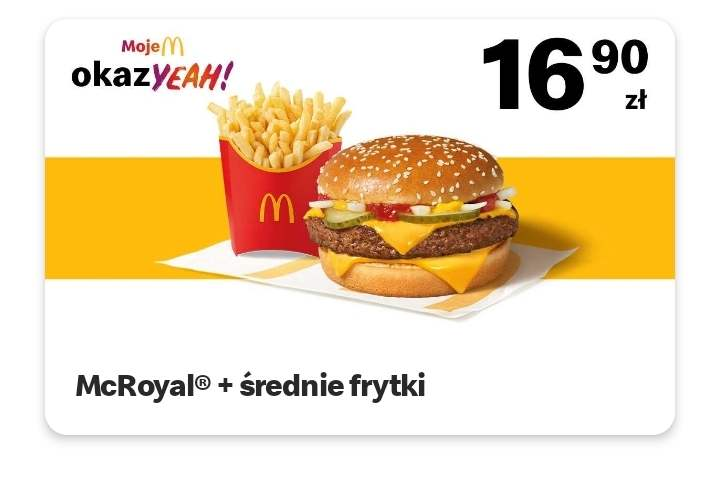
\includegraphics[width=\linewidth]{coupon1.jpg}
        \caption{The example coupon from fast-food restaurants chain mobile application}
    \end{minipage}
    \hfill
    \begin{minipage}{0.45\textwidth}
        \centering
        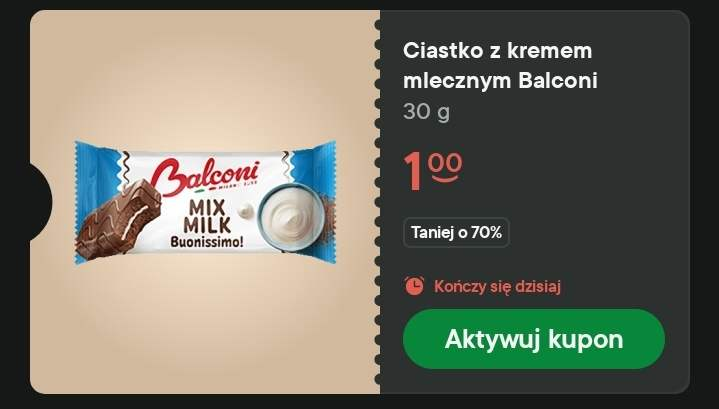
\includegraphics[width=\linewidth]{coupon2.jpg}
        \caption{The example coupon from grocery store mobile application}
    \end{minipage}
    \caption{The example digital coupons}
    \label{fig:example_coupons}
\end{figure}


\subsection{Our data model of digital coupon}
\label{sec:coupon_model}
In the following research we model a digital coupon as a collection of named fields:
\begin{enumerate}
    \item \textit{product\_name}: the name of the product
    \item \textit{valid\_unitl}: the text representing the date of coupon expiration
    \item \textit{discount\_text}: the text representing the discount offered to the user
    \item \textit{activated}: either true or false, indicates whether the coupon has been activated
\end{enumerate}
We will allow for special \textit{null} value in the above fields in case no data is available.

An example of a digital coupon represented in JSON format is shown below:

\begin{lstlisting}[language=json, caption={Example of a digital coupon in JSON format}, label={lst:coupon_example}]
{
    "product_name": "Shampoo X",
    "valid_unitl": "2025-06-30",
    "discount_text": "20% OFF",
    "activated": true
}
\end{lstlisting}

\subsection{Collection of Statistics Related to Digital Coupons}
Given the significance of digital coupons in contemporary marketing strategies \cite{targeted_reminders}, analyzing their lifecycle is essential. To facilitate such analyses, researchers collect various statistical metrics, including the fraction of redeemed coupons among all distributed coupons referred henceforth as redemption rate \cite{danaher2015} and customer engagement \cite{jayadharshini2023}, while also assessing their impact on sales performance \cite{jayadharshini2023}.

\subsubsection{Redemption Rate}
The measurement of coupon redemption rates is primarily based on either survey data \cite{nayal2021} or controlled experimental studies \cite{danaher2015}. However, the company Murmuras \cite{murmuras} has introduced an alternative approach that enables the direct collection of coupon-related data from users' devices. This method utilizes a screen content scraping tool installed on the devices. Additionally, the tool has the ability to record user's actions.  Having access to all the user's interactions and visual changes in the layout, it is possible to detect the coupon redemption. This allows for large-scale data acquisition while reducing the costs associated with traditional survey-based methods.

\subsubsection{Customer Engagement and Impact on Sales}

Customer engagement metrics, such as conversion rates and the effect of e-coupon issuance on sales, can potentially be measured using statistical analysis tools operating on the seller's website~\cite{seo2023}. The conversion rate is typically derived by tracking visitor activity, while the impact on sales is estimated by correlating the updated conversion rate with the frequency of coupon issuance.

Although this approach provides valuable insights, it relies on direct collaboration with the coupon issuer and is constrained to a single webpage. Consequently, it is not applicable to our study, as we aim to analyze arbitrary mobile applications with diverse coupon designs.

\section{Project background and motivation}
With the rapid advancement of information technology, the Internet has become one of the most crucial facets for many businesses to perform marketing activities \cite{design_of_coupons}. One of the key marketing tools in business-to-consumer (B2C) e-commerce is the digital coupon (also referred to as an electronic coupon) \cite{targeted_reminders}. In comparison to paper coupons, digital coupons are characterized by their wide reach, rapid distribution, and low spread costs. Furthermore, a key advantage of digital coupons is their ability to facilitate targeted marketing by offering personalized discounts to different customers, thereby increasing sales \cite{design_of_coupons}. To maximize the benefits of digital coupons, it is essential for businesses to assess the effectiveness of their coupon campaigns, evaluate their reach, and analyze their competitors’ strategies. By tracking key performance metrics such as redemption rates, customer engagement, and sales impact, businesses can refine their marketing approaches to optimize results. Additionally, studying competitors' digital coupon strategies enables businesses to identify market trends, adjust their promotional tactics, and maintain a competitive edge in the evolving digital marketplace.

Large Language Models (LLMs) have become a fundamental technique in contemporary machine learning, replacing previously utilized recurrent neural network (RNN) architectures in the field of natural language processing (NLP) \cite{li2024}. Subsequent research has demonstrated their applicability to structured input data \cite{sui2024}. Additionally, there have been efforts to integrate these models into web scraping pipelines \cite{scapegraph_repo}.

Recent statistics underscore the significance of mobile devices in the domain of coupon distribution. For example, studies have shown that over 90\% of digital coupon users access their vouchers via smartphones \cite{emarketer_coupon_stats}, and similar figures are reported by other industry sources \cite{coupon_stats_2}. This high rate of mobile usage creates a pressing need for coupon analysis tools that are optimized for mobile platforms, ensuring that consumers receive timely and personalized offers regardless of their location or device.

In light of these trends, the company Murmuras has tasked us with developing a solution based on a machine learning model that can be deployed as a mobile application. This model will process input representing the user's onscreen view and extract digital coupons along with their relevant data. This solution must be capable of running locally on the device, ensuring efficient processing without relying on external servers. By leveraging advanced machine learning techniques, the app will handle the diverse formats and layouts of digital coupons, thereby facilitating the collection of data regarding coupons.

\section{Problem Statement}

The objective of this work is to extract coupons visible to the user from the content displayed on a mobile device screen. The extracted coupons should be represented as a JSON list, with each entry conforming to the format specified in Section~\ref{sec:coupon_model}.

The screen content is provided in the form of a \texttt{.CSV} file, which encodes an XML tree structure representing the underlying screen layout. Each row in this file corresponds to a single view element within the screen hierarchy~\cite{android_view}. The dataset includes at least the following attributes:

\begin{enumerate}
    \item \textbf{view\_depth}: The depth of the view within the XML tree hierarchy.
    \item \textbf{text}: The textual content displayed to the user within the view.
    \item \textbf{id}: A unique identifier for a screen sample. Each sample consists of a set of views observed either simultaneously or in directly consecutive snapshots.
    \item \textbf{time}: The timestamp indicating when the view was recorded.
    \item \textbf{view\_id}: The unique identifier assigned to the view by the Android API.
\end{enumerate}

An example of the dataset to illustrate described format is provided in Table~\ref{tab:dataset_example}.

\begin{table}[h]
    \centering
    \begin{tabular}{|c|c|c|c|c|}
        \hline
        \textbf{view\_depth} & \textbf{text} & \textbf{id} & \textbf{time} & \textbf{view\_id} \\
        \hline
        2 & "50\% OFF" & 101 & 12:30:15 & \texttt{com.example.app:id/discount\_label} \\
        3 & "Buy 1 Get 1 Free" & 101 & 12:30:15 & \texttt{com.example.app:id/promo\_banner} \\
        2 & "Limited Offer" & 102 & 12:31:05 & \texttt{com.example.app:id/offer\_text} \\
        \hline
    \end{tabular}
    \caption{Example of dataset format representing screen content.}
    \label{tab:dataset_example}
\end{table}

Additional requirement is that the screen content processing will be performed exclusively on the end device to mitigate potential privacy concerns.

\section{Project goals}
\begin{enumerate}
    \item A tool to process the data extracted from the device into a format suitable for use by the model.
    \item A machine learning tool for extracting the data that is of interest to us, such as the coupon name, expiration dates, prices, etc. The model should be capable of handling various coupon formats and layouts with high accuracy.
    \item An optional tool for post-processing the output data from the tool mentioned in the previous point into a common format.
    \item An application that runs the above three tools on a mobile device. (Optional)
    \item A key requirement is that the machine learning model must be deployable on the mobile device itself to guarantee data privacy.
\end{enumerate}

\section{Potential applications of the project}
\subsection{Assessing coupon effectiveness}
The access to the content of mobile device screen allows us to list all the coupons seen by the user. Additionally, as we will retrieve information about coupon activation status, there will be possibility to track coupon redemptions by comparing the coupons models \textit{active} field.

Given that, our solution will aid businesses in analyzing consumer behavior and optimizing their marketing strategies. By facilitating the collection of data on coupon characteristics and their redemption rates, businesses will be able to assess the effectiveness of their coupon campaigns—determining whether they achieve the desired results. Additionally, large-scale analysis of coupon data can reveal valuable insights into purchasing patterns, preferred discount types, and the most appealing products or services.

\subsection{Market analysis and competitor monitoring}
The machine learning is proven to be a useful tool in the field of market competitors analysis but it requires significant amounts of data\cite{competitor_tariffs}.
The aforementioned gathering of data about displayed coupons can also be utilized in further monitoring of competitors' coupon strategies, their effectiveness, and whether they provide better discounts. Using machine learning to identify and analyze competitors' strategies is more cost-effective compared to exhaustive web scraping or mystery shopping \cite{competitor_tariffs}. This will enable businesses to make better informed decisions about their own marketing campaigns and provide a comprehensive understanding of the competitive landscape.

\chapter{Machine learning and the dangers associated with it}
Note: this chapter is a work in progress, bullet points aim to provide guidance when writing this section

(1) What is the difference between machine learning, artificial intelligence, and deep learning? \\
(1a) Provide the definitions/a brief explanation of each of the above.\\
(1b) Explain what a benchmark is and what it is used for. \\

\subsection{Benchmark}
Benchmarking is the process of running a set of, among others, computer programs against a set of tests to assess their relative performance or precision \cite{benchmark}.

(2) Understanding ML models \\
(2a) Explain what a model is \\
(2b) Explain how a model works, how it is trained, datasets, linear regression, supervised vs unsupervised learning (?), federated learning (?), computer vision (?) \\
(2c) What is quantization and why it is this of interest to us \\

(3) What is NLP \\
(3a) Explain what NLP is and why it is of interest to us for this project \\
(3b) BERT, Llama, ChatGPT and other models (briefly explain their differences, advantages and disadvantages, paramters, memory usage (?)) \\

(4) Should we be scared of AI? \\
(4a) https://www.youtube.com/watch?v=yh1pF1zaauc. (from our mentor) \\
(4b) Privacy and ethics of data collection and processing (present the problem, why people are concerned about this, then later on in the document we say that we resolved this issue because we are processing the data locally etc) \\
(4c) Adversarial attacks (I'm not sure this is particularly relevant to our project but it mught be worth mentioning) \\
(4e) Accuracy concerns, how can we be sure that our model is correct? Lack of human oversight \\
(4f) Environmental concerns
// HF tutorial: env concerns => fine tune not training



\chapter{Overview of Existing Solutions}

To the best of our knowledge, at the time of this project's commissioning, no publicly available solutions directly addressed this problem. The most comparable approaches involve existing multimodal models. While widely used models such as ChatGPT and Gemini provide general data extraction capabilities~\cite{brinkmann2023}, they are unsuitable for our task due to their substantial computational requirements. A key limitation of these models is their large size—for example, GPT-3 consists of 175 billion parameters\cite{chatgpt_params}—rendering them impractical for deployment on mobile devices~\cite{LinguaLinked}.

Alternatively, computer vision models can be used to extract text and bounding boxes from screen images. Microsoft’s OmniParser~\cite{omniparser_intro}, for instance, has demonstrated strong performance on the ScreenSpot dataset~\cite{omniparser_intro, cheng2024}. However, the challenge of organizing extracted text into structured coupon data renders this approach unsuitable for our study. Furthermore, our experiments with running OmniParser locally on example images indicate that it relies on CUDA technology, making it impractical for deployment on mobile devices.

\section{Murmuras' existing solution}
Murmuras' current approach relies on a set of fixed scrapping programms tailored to specific layouts from limited set of applications, making it inflexible and expansive to generalize across diverse coupon formats. This lack of adaptability limits its usefulness in real-world scenarios where coupon structures vary widely. Since our goal is to develop a solution that is easily adaptable for processing diverse mobile content, this method is not well-suited for our needs.

In contrast, Murmuras' most-recent proof of concept involves wrapping the \texttt{CSV} data with a prompt that instructs the model and sending it to GPT-4o-mini. This approach leverages an LLM to interpret the data to extract relevant coupon details. However, the reliance on an external server means the solution does not run locally on the mobile device, leading to potential privacy concerns, latency issues, and a dependence on internet connectivity.

\section{Scapegraph AI}
ScrapeGraphAI is an open-source library that streamlines data extraction from websites and local documents by utilizing LLMs and graph logic to construct scraping pipelines \cite{scapegraph_repo}. The library supports integration with various LLMs, including local models through the use of Ollama \cite{ollama_repo} \cite{scapegraph_usage}.

However, Scrapepraph AI provides only Python and Node.js SDKs \cite{scapegraph_sdks}, which could prove to be an issue with regard to mobile deployment, because neither Python nor Node.js is natively supported on iOS or Android \cite{android_dev_site} \cite{ios_dev_site}.

Moreover, due to mobile devices typically having limited processing power and memory compared to desktop computers or servers \cite{mobile_resources}, we cannot solely rely on the size of the model in order to improve performance. We believe that through fine-tuning LLMs, we are able to develop tools that are far more viable for edge device usage.

\chapter{Technologies}

\section{General}

The main platforms used during the development process were Hugging Face\cite{hugging-face} and GitHub\cite{github}. Hugging Face served as a hub for storing and managing both trained machine learning models and datasets. During development, we also made extensive use of several Python libraries provided by Hugging Face, including \textit{datasets}\cite{lhoest2021datasetscommunitylibrarynatural}, \textit{transformers}\cite{wolf-etal-2020-transformers}, and \textit{evaluate}\cite{evaluate}. GitHub, in turn, offered version control for our code and documentation, and supported DevOps tasks such as issue tracking and automated unit testing.

Python\cite{python} was the primary programming language used, due to its broad support for machine learning workflows. Additionally, some auxiliary experiments related to Android deployment were conducted using Kotlin\cite{kotlin}\cite{service_demo_app_repo}.

\section{LLaMA Proposal}

Our first solution was based on the LLaMA architecture and utilized a custom fine-tuned version of LLaMA-3.2-1b provided by Meta\cite{meta-llama}. Fine-tuning was performed using the Unsloth\cite{unsloth} tool, which enabled efficient resource usage. Specifically, Unsloth applied the LoRA (Low-Rank Adaptation) fine-tuning technique\cite{hu2021loralowrankadaptationlarge}, reducing the number of trainable parameters to approximately 10 million. It also facilitated easy model conversion to the GGUF format.

The fine-tuning process was carried out on the Modal platform\cite{modal}, which allowed us to define execution environments directly in Python and execute code on cloud infrastructure equipped with H100 GPUs. Training progress and logs were monitored using Weights \& Biases (Wandb)\cite{wandb}.

Model inference was conducted using the Llama.cpp\cite{llama-cpp} tool, utilizing the model converted to the GGUF format.

\section{BERT Proposal}

The second approach—a two-stage BERT pipeline—was also trained on the Modal platform. Logging and experiment tracking were similarly managed using Wandb.

\section{Auxiliary Experiments}

Additional experiments conducted as part of this project involved frameworks such as SpaCy\cite{spacy}\cite{spacy-exp} and Scrapegraph AI\cite{scapegraph_repo}\cite{scrapegraph-exp}, as well as mobile deployment tools including ONNX\cite{onnx}\cite{onnx-exp}, liteRT\cite{lite-rt}\cite{lite-rt-exp}, and Executorch\cite{executorch}\cite{executorch-exp}. These experiments were developed using Android Studio\cite{android-studio}\cite{service_demo_app_repo} and Jupyter notebooks\cite{jupyter}, running in an IPython\cite{ipython} environment.


% \section{}

% \chapter{Technologies}
% \chapter{Architecture design}
% \chapter{Performance}
% \chapter{Possible extensions}
% \chapter{Summary}
% \chapter{Charts}



\begin{thebibliography}{99}

\addcontentsline{toc}{chapter}{Bibliography}

\bibitem{murmuras}
\textit{Murmuras website}.
\url{https://murmuras.com/}.
[Accessed 2025-02-11].

\bibitem{coupon_definition}
\textit{Britannica Dictionary definition of COUPON}.
\url{https://www.britannica.com/dictionary/coupon}.
[Accessed 2025-02-03].

\bibitem{benchmark}
\textit{Computer Benchmark}.
\url{https://bhatabhishek-ylp.medium.com/benchmarking-in-computer-c6d364681512}.
[Accessed 2025-02-03].

\bibitem{design_of_coupons}
Xiong Keyi, Yang Wensheng
\textit{Research on the Design of E-coupons for Directional Marketing of Two Businesses in Competitive Environment}.
\url{https://www.sciencepublishinggroup.com/article/10.11648/j.ijefm.20200801.16}.
[Accessed 2025-02-04].

\bibitem{targeted_reminders}
Li Li, et. al.
\textit{Targeted reminders of electronic coupons: using predictive analytics to facilitate coupon marketing}.
\url{https://link.springer.com/article/10.1007/s10660-020-09405-4}.
[Accessed 2025-02-04].

\bibitem{competitor_tariffs}
Bernhard König, et. al.
\textit{Analysing competitor tariffs with machine learning}.
\url{https://www.milliman.com/en/insight/analysing-competitor-tariffs-with-machine-learning}.
[Accessed 2025-02-04].

\bibitem{ml_general}
Iqbal H. Sarker
\textit{Machine Learning: Algorithms, Real-World Applications and Research Directions}.
\url{https://link.springer.com/article/10.1007/s42979-021-00592-x}.
[Accessed 2025-02-05].

\bibitem{emarketer_coupon_stats}
Sara Lebow
\textit{How consumers access digital coupons}.
\url{https://www.emarketer.com/content/how-consumers-access-digital-coupons}.
[Accessed 2025-02-05].

\bibitem{coupon_stats_2}
\textit{Unveiling IT Coupons Trends and Statistics}.
\url{https://www.go-globe.com/unveiling-it-coupons-trends-statistics/}.
[Accessed 2025-02-05].

\bibitem{chatgpt_params}
\textit{Tom B. Brown, Benjamin Mann, Nick Ryder, Melanie Subbiah, Jared
Kaplan, Prafulla Dhariwal, Arvind Neelakantan, Pranav Shyam, Girish
Sastry, Amanda Askell, Sandhini Agarwal, Ariel Herbert-Voss, Gretchen
Krueger, Tom Henighan, Rewon Child, Aditya Ramesh, Daniel M.
Ziegler, Jeffrey Wu, Clemens Winter, Christopher Hesse, Mark Chen,
Eric Sigler, Mateusz Litwin, Scott Gray, Benjamin Chess, Jack Clark,
Christopher Berner, Sam McCandlish, Alec Radford, Ilya Sutskever, and
Dario Amodei. Language models are few-shot learners, 2020}
// Would be great to get the link and change this into APA

\bibitem{scapegraph_intro}
Satyam Tripathi
\textit{ScrapeGraphAI Tutorial - Getting Started with LLMs Web Scraping}
\url{https://scrapingant.com/blog/scrapegraphai-llms-web-scraping}

\bibitem{omniparser_intro}
\textit{Yadong Lu, Jianwei Yang, Yelong Shen, and Ahmed Awadallah. Omni-
parser for pure vision based gui agent, 2024.}

\bibitem{gh_issue_810_scapegraph}
\textit{Can not Set Model Tokens to Local Model with OpenAI API Format \#810}
\url{https://github.com/ScrapeGraphAI/Scrapegraph-ai/issues/810}

\bibitem{gh_issue_752_scapegraph}
\textit{Can't load tokenizer for 'gpt2' \#752}
\url{https://github.com/ScrapeGraphAI/Scrapegraph-ai/issues/752}

\bibitem{mobile_resources}
Xiang Li, et. al.
\textit{Large Language Models on Mobile Devices: Measurements, Analysis, and Insights}
\url{https://dl.acm.org/doi/10.1145/3662006.366205}

\bibitem{LinguaLinked}
Junchen Zhao, et. al.
\textit{LinguaLinked: A Distributed Large Language Model Inference System for Mobile Devices}
\url{https://arxiv.org/pdf/2312.00388}

\bibitem{sequence_matcher}
\textit{difflib — Helpers for computing deltas}
\url{https://docs.python.org/3/library/difflib.html}

\bibitem{meta-llama}
\textit{Llama 3.2 published by Meta}
\url{https://ai.meta.com/blog/llama-3-2-connect-2024-vision-edge-mobile-devices/}
[Accessed 2025-04-17]

\bibitem{unsloth}
\textit{Unsloth}
\url{https://unsloth.ai/}
[Accessed 2025-04-17]

\bibitem{hugging-face}
\textit{The Hugging Face Platform}
\url{https://huggingface.co/}
[accessed 17.04.2025]

\bibitem{github}
\textit{The Github platform}
\url{https://github.com/}
[accessed 17.04.2025]

\bibitem{modal}
\textit{The Modal platform}
\url{https://modal.com/}
[accessed 17.04.2025]

\bibitem{wandb}
\textit{The Wandb platform}
\url{https://wandb.ai/}
[accessed 17.04.2025]

\bibitem{python}
\textit{The website of Python programming language}
\url{https://www.python.org/}
[accessed 17.04.2025]

\bibitem{service_demo_app_repo}
\textit{Our experiment with mobile app that runs in background}
\url{https://github.com/ZPP-MURMURAS/ZPP_Murmuras/tree/main/research/service_demo_app}

\bibitem{kotlin}
\textit{Webpage of the Kotlin programming Language}
\url{https://kotlinlang.org/}
[accessed 24.04.2025]

\bibitem{hu2021loralowrankadaptationlarge}
\textit{dward J. Hu and Yelong Shen and Phillip Wallis and Zeyuan Allen-Zhu and Yuanzhi Li and Shean Wang and Lu Wang and Weizhu Chen (2021): LoRA: Low-Rank Adaptation of Large Language Models}
\url{https://arxiv.org/abs/2106.09685}

\bibitem{triton}
\textit{Tillet, Philippe and Kung, H. T. and Cox, David (2019): Triton: an intermediate language and compiler for tiled neural network computations}
\url{https://doi.org/10.1145/3315508.3329973}

\bibitem{lhoest2021datasetscommunitylibrarynatural}
\textit{Lhoest et al (2021): Datasets: A Community Library for Natural Language Processing}
\url{https://arxiv.org/abs/2109.02846}

\bibitem{evaluate}
\textit{evaluate Python library}
\url{https://pypi.org/project/evaluate/}
[accessed 24.05.2025]

\bibitem{wolf-etal-2020-transformers}
\textit{Wolf et al (2020): Transformers: State-of-the-Art Natural Language Processing}
\url{https://aclanthology.org/2020.emnlp-demos.6/}

\bibitem{llama-cpp}
\textit{Llama.cpp repository}
\url{https://github.com/ggml-org/llama.cpp}
[Accessed 25.04.2025]

\bibitem{spacy}
\textit{SpaCy Python library}
\url{https://pypi.org/project/spacy/}
[Accessed 25.04.2025]

\bibitem{onnx}
\textit{ONNX framework}
\url{https://github.com/onnx/onnx}
[Accessed 25.04.2025]

\bibitem{lite-rt}
\textit{LiteRT environment}
\url{https://ai.google.dev/edge/litert}
[Accessed 25.04.2025]

\bibitem{executorch}
\textit{ExecuTorch framework}
\url{https://pytorch.org/executorch-overview}
[Accessed 25.04.2025]

\bibitem{android-studio}
\textit{Android Studio webpage}
\url{https://developer.android.com/studio}
[Accessed 25.04.2025]

\bibitem{jupyter}
\textit{Jupyter Notebook Webpage}
\url{https://jupyter-notebook.readthedocs.io/en/stable/}
[Accessed 25.04.2025]

\bibitem{ipython}
\textit{IPython Kernel Webpage}
\url{https://ipython.org/}
[Accessed 25.04.2025]

\bibitem{spacy-exp}
\textit{Overview od spacy}
\url{https://github.com/ZPP-MURMURAS/ZPP_Murmuras/tree/main/research/spacy_research}
[Accessed 25.04.2025]

\bibitem{scrapegraph-exp}
\textit{Experiments with Scrapegraph AI}
\url{https://github.com/ZPP-MURMURAS/ZPP_Murmuras/tree/main/research/scrapegraphai}
[Accessed 25.04.2025]

\bibitem{onnx-exp}
\textit{Demonstrative mobile deployment of a model in ONNX/ framework.}
\url{https://github.com/ZPP-MURMURAS/ZPP_Murmuras/tree/main/research/onnx_demo_app}
[Accessed 25.04.2025]

\bibitem{lite-rt-exp}
\textit{Demostrative mobile deployment of LiteRT model.}
\url{https://github.com/ZPP-MURMURAS/ZPP_Murmuras/tree/main/research/litert_deployment}
[Accessed 25.04.2025]

\bibitem{executorch-exp}
\textit{Overview of ExecuTorch suitability in our problem.}
\url{https://github.com/ZPP-MURMURAS/ZPP_Murmuras/blob/main/research/executorch/executorch_llama_report.md}
[Accessed 25.04.2025]

\end{thebibliography}

\end{document}


%%% Local Variables:
%%% mode: latex
%%% TeX-master: t
%%% coding: latin-2
%%% End:
